\section{Theoretical Analysis}
\label{sec:analysis}

In this section, the circuit shown in \textbf{Figure~\ref{fig:diagram_t3}} is analysed
theoretically.
\begin{figure}[H] \centering
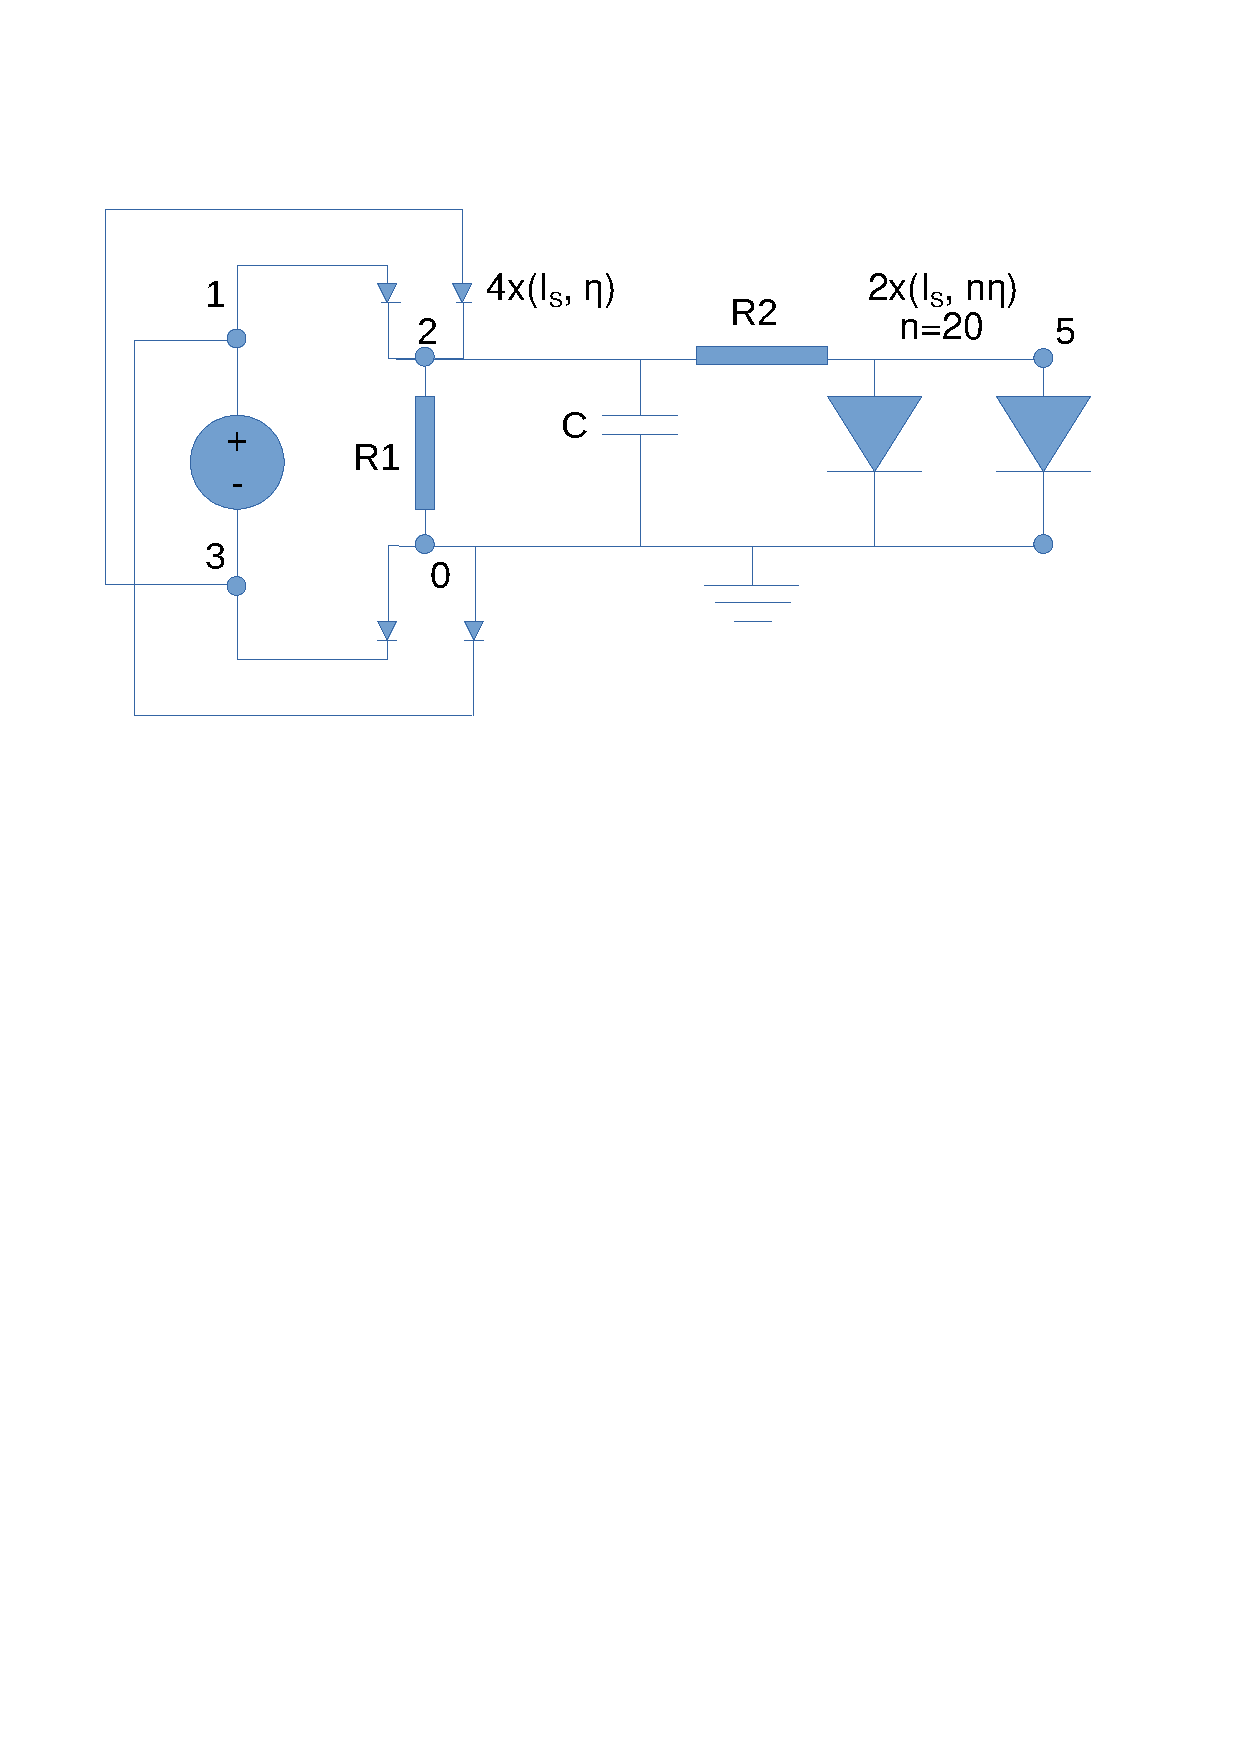
\includegraphics[width=0.6\linewidth]{diagram_t3.pdf}
\caption{Diagram of the circuit considered for the computations and simulations}
\label{fig:diagram_t3}
\end{figure}

%point 1
\subsection{Analysis for $t<0$} 
The nodal method is aplied to the circuit in order to determine the voltage in all nodes and the current on all branches . The nodal method aplies KVL and for $t<0$ no current passes through the capacitor, and therefore this component behaves like an open circuit.
%In \textbf{Table~\ref{tab:theoretical}} the values for the branch currents and the node voltages obtained from the Octave script for both methods are presented. Here, the node voltages in the mesh method were computed from the respective currents, which were determined as described in the previous subsection.





%\begin{figure}[H] \centering
%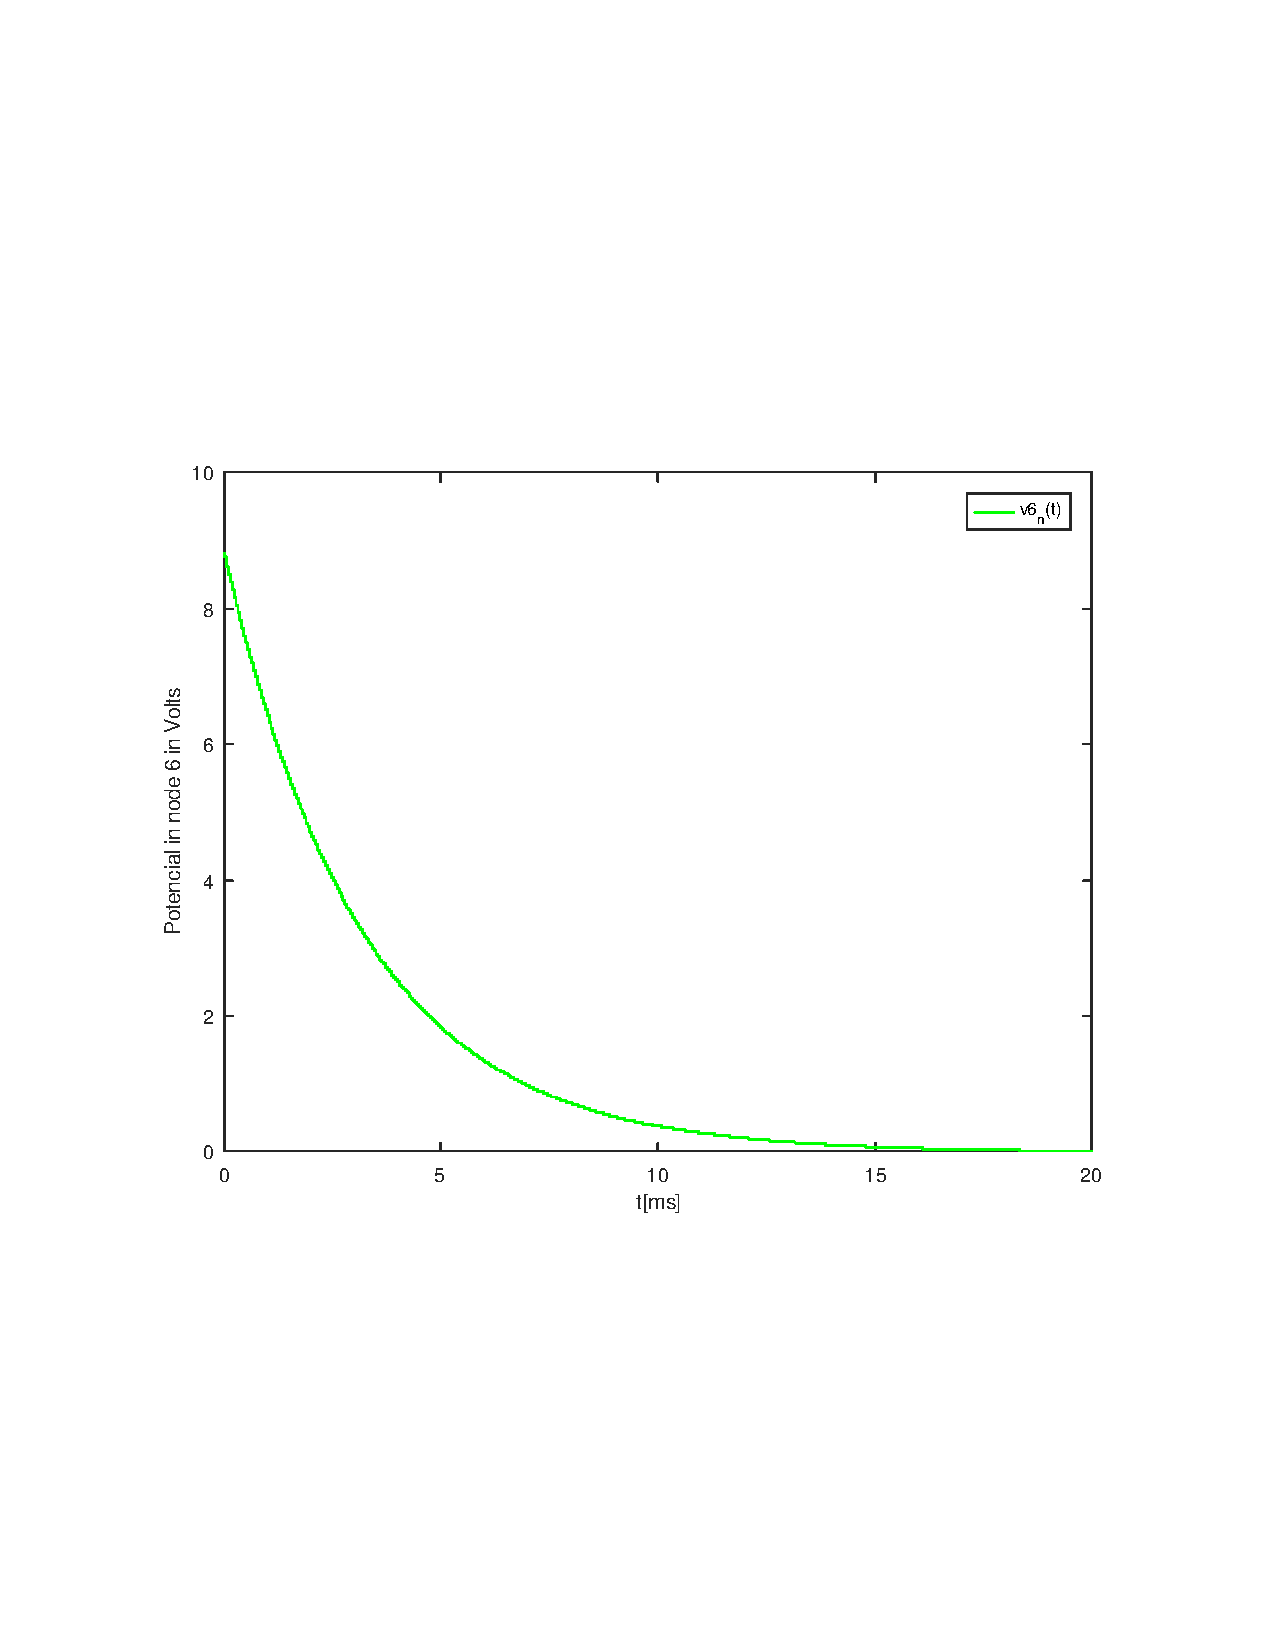
\includegraphics[width=0.9\linewidth]{natural_tab.pdf}
%\caption{Natural response of $V_6$ as a function os time in the interval from [0,20] ms}
%\label{fig:natural}
%\end{figure} 



%\begin{figure}[H] \centering
%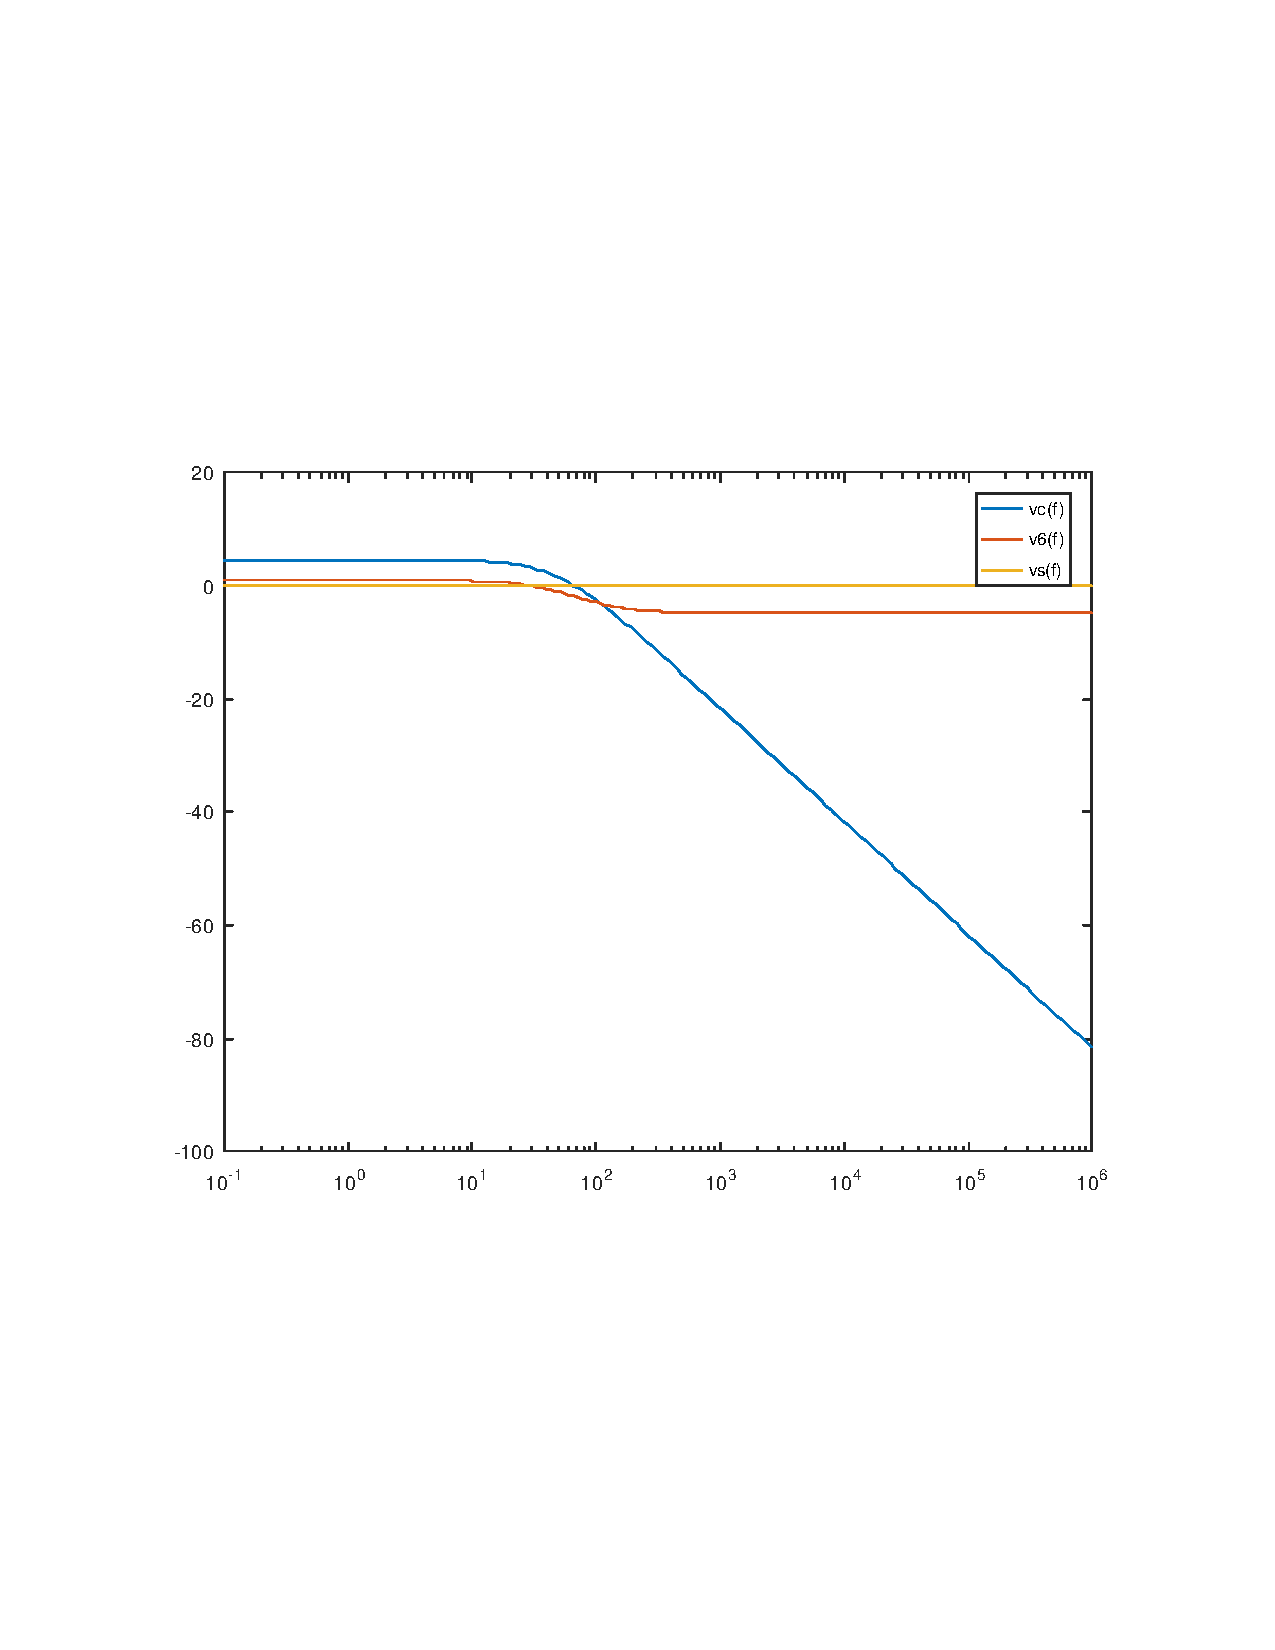
\includegraphics[width=0.9\linewidth]{freq_resp_tab.pdf}
%\caption{Graph for amplitude frequency response, in dB, of $V_c$, $V_6$ and $V_s$ for frequencies ranging from 0.1Hz to 1MHz (logarithmic scale).}
%\label{fig:freq_resp}
%\end{figure}




\pagebreak


